% ============================================================
%  深圳大学实验报告（SZU Experiment Report Template）
%  Project 1: NumPy re-implementation of the OpenCLIP ViT-B-32 vision tower
%  Compile with XeLaTeX
% ============================================================

\documentclass[a4paper,12pt]{article}

% ----------------------------
% 中文与字体支持
% ----------------------------
\usepackage{fontspec}
\usepackage{xeCJK}
\IfFontExistsTF{Noto Serif CJK SC}
  {\setCJKmainfont{Noto Serif CJK SC}}
  {\setCJKmainfont{SimSun}[BoldFont=SimHei]}
\setmonofont{Consolas}[Scale=0.88]

% ----------------------------
% 页面设置与常用宏包
% ----------------------------
\usepackage{geometry}
\geometry{left=1in, right=1in, top=1in, bottom=1in}

\usepackage{longtable}
\usepackage{graphicx}
\usepackage{fancyhdr}
\usepackage{tikz}
\usetikzlibrary{calc}
\usepackage{verbatim}
\usepackage{float}
\usepackage{array}
\usepackage{amsmath}
\usepackage{amssymb}
\usepackage[labelsep=quad, font=small, labelfont=bf]{caption}
\usepackage[hidelinks]{hyperref}

\graphicspath{{figs/}}

\fancyhf{}
\fancyhead[C]{}
\fancyhead[R]{}
\pagestyle{plain}

% 中文图表标题，与正文表述一致
\renewcommand{\figurename}{图}
\renewcommand{\tablename}{表}

\setlength{\parskip}{1.5pt}
\setlength{\abovedisplayskip}{3pt}
\setlength{\belowdisplayskip}{3pt}
\renewcommand{\arraystretch}{1.05}

% ============================================================
%                      文档开始
% ============================================================

\begin{document}

% ============================================================
% 封面页
% ============================================================
\begin{titlepage}
    \centering
    \vspace*{2cm}
    \Huge{\textbf{深 \ 圳 \ 大 \ 学 \ 实 验  \ 报 \ 告}}\\[1.5cm]

    {\Large\textbf{课程名称}\quad\underline{\makebox[8cm][c]{Python程序设计}}}\\[0.5cm]
{\Large
\noindent\makebox[3.2cm][l]{\textbf{项目名称}}
\underline{\makebox[8cm][c]{\small NumPy 复现 CLIP 视觉编码器}}}\\[0.5cm]
{\Large
\noindent\makebox[3.2cm][l]{\textbf{学 \quad \quad 院}}
\underline{\makebox[8cm][c]{人工智能学院}}}\\[0.5cm]
{\Large
\noindent\makebox[3.2cm][l]{\textbf{专 \quad \quad 业}}
\underline{\makebox[8cm][c]{}}}\\[0.5cm]
{\Large
\noindent\makebox[3.2cm][l]{\textbf{指导教师}}
\underline{\makebox[8cm][c]{舒婷}}}\\[0.5cm]
{\Large
\noindent\makebox[3.2cm][l]{\textbf{报 \quad 告 \quad 人}}
\underline{\makebox[3cm][c]{}}
\hspace{0.5cm}
\textbf{学号}
\underline{\makebox[3cm][c]{}}}\\[0.5cm]
{\Large
\noindent\makebox[3.2cm][l]{\textbf{实验时间}}
\underline{\makebox[8cm][c]{}}}\\[0.5cm]
{\Large
\noindent\makebox[3.2cm][l]{\textbf{提交时间}}
\underline{\makebox[8cm][c]{}}}\\[1.5cm]

    \vfill
    \Large{\textbf{教务处制}}
\end{titlepage}

\newpage

% ============================================================
% 正文部分
% ============================================================

\section{Objectives}

本实验的目标是在不使用 PyTorch、OpenCLIP 包与 GPU 的前提下，仅用 NumPy 实现 OpenCLIP
ViT-B-32 视觉塔的前向计算，使输出与独立生成的 FP32 参考实现逐元素一致。模型参数由课程提供并固定，
实验中不涉及训练或参数更新，属于前向复现而非模型训练。

输入为经给定预处理（最短边缩放到 224、双三次插值、中心裁剪、CLIP 均值/方差归一化）后的 float32
图像批 \texttt{[B,3,224,224]}；输出为每张图像一个 512 维单位长度向量 \texttt{[B,512]}。判定条件为
形状一致、dtype 为 float32、无 NaN/Inf，且
\(|\Delta| \le \mathrm{atol} + \mathrm{rtol}\cdot|\mathrm{ref}|\)（output 阶段 atol=2e-5、rtol=2e-4）。

结构固定为：patch 32$\times$32（$224/32=7$，共 49 块）、token 数 $N=50$（1 个 CLS + 49 个 patch）、
宽度 $D=768$、头数 $H=12$、头维 $d_h=64$、12 个 Transformer 块、MLP 中间宽度 3072、输出维度 512。
数据为课程提供的 10 张图片与 \texttt{weights/image\_encoder.npz} 中的 152 个视觉张量
（87{,}849{,}216 个参数，SHA-256 逐张量校验）。

验证手段是课程脚本 \texttt{check.py} 的八阶段对拍（assets、preprocess、patches、tokens、block0、
last\_tokens、output、batch）；其中 batch 阶段打乱顺序并重复同一张图，用于检验实现是否与批次顺序
无关、是否存在跨样本状态。

\section{Overview}

整体思路是把一次前向拆成若干“只做一件事”的形状变换，每一步都能单独与参考数组对拍，从而把调试
范围限定在最小环节（图~\ref{fig:pipeline}）。编码器共 12 层，每层含注意力与 MLP 两条 pre-LN 残差
支路；本实验只取 CLS 位置的输出并投影到 512 维，不接分类头。

\begin{figure}[H]
    \centering
    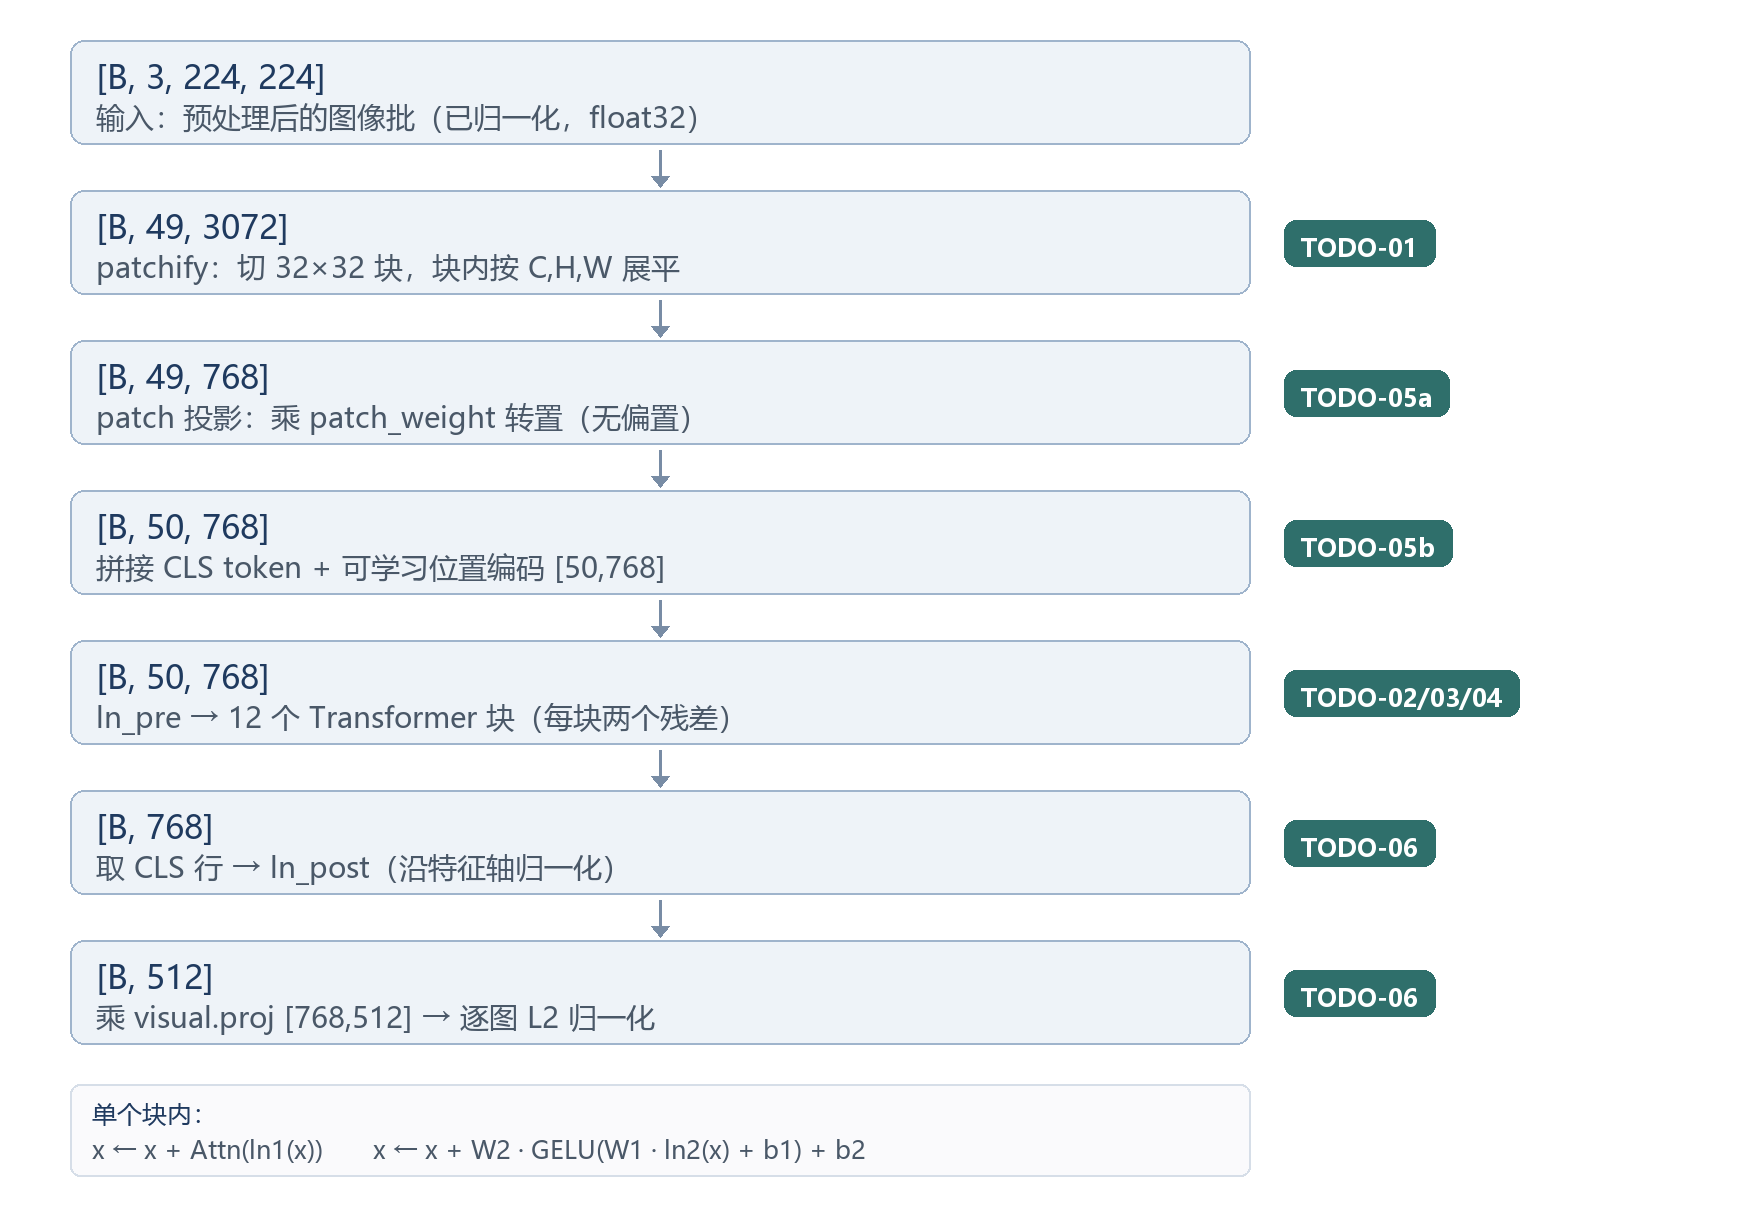
\includegraphics[width=0.88\linewidth]{pipeline.png}
    \caption{本实验的张量形状流水线（ViT 视觉塔），右侧标注对应实现位置（TODO-01～TODO-06）。}
    \label{fig:pipeline}
\end{figure}

\begin{enumerate}
    \item[Spot 1] \textbf{切块}：把 32$\times$32、步长 32 的卷积等价视为切块，
          \texttt{[B,3,224,224]} $\rightarrow$ \texttt{[B,49,3072]}；
    \item[Spot 2] \textbf{投影 + CLS + 位置}：patch 行乘 \texttt{conv1} 权重得到
          \texttt{[B,49,768]}，拼接 CLS 并加可学习位置编码后为 \texttt{[B,50,768]}；
    \item[Spot 3] \textbf{十二个 pre-LN 双残差块}：每块含注意力与 MLP 两条支路，形状恒为
          \texttt{[B,50,768]}；
    \item[Spot 4] \textbf{输出头}：取 CLS 行、做 \texttt{ln\_post}、乘 \texttt{visual.proj}，
          再逐图 L2 归一化得到 \texttt{[B,512]}。
\end{enumerate}

单块算术与 helpers.py 给定的 LayerNorm、精确 GELU、softmax 组合如下，实验中只需正确实现线性层、
头拆分与残差的组合方式：
\begin{align}
\mathrm{LN}(x) &= \frac{x-\mu}{\sqrt{\sigma^2+10^{-5}}}\,\gamma+\beta, \label{eq:ln}\\
A &= \mathrm{softmax}\!\left(\frac{QK^{\top}}{\sqrt{d_h}}\right),\quad
\text{Context}=A V,\quad [Q,K,V]=\mathrm{LN}(x)W_{qkv}+b_{qkv}, \label{eq:attn}\\
x &\leftarrow x+\mathrm{Attn}\big(\mathrm{LN}_1(x)\big),\quad
x \leftarrow x+W_2\,\mathrm{GELU}\big(W_1\mathrm{LN}_2(x)+b_1\big)+b_2, \label{eq:block}\\
\mathrm{out} &= \mathrm{unit}\big(\mathrm{LN}_{post}(x_0)\cdot P\big),\quad P\in\mathbb{R}^{768\times512}.
\label{eq:out}
\end{align}

\section{Implementations}

\subsection{复现环境与运行步骤}

全部计算在单机 CPU 上完成，依赖仅 NumPy 与 Pillow（表~\ref{tab:env}）。依次执行
\texttt{pip install -r requirements.txt}、\texttt{check.py -{}-stage all} 与
\texttt{run.py -{}-output output\_tokens.npz}；脚本按自身路径定位模型与图片，可在任意工作目录运行。
\texttt{check.py} 的退出码 0/1/2 分别表示全部通过、数值不符、仍有未实现的 TODO。

\begin{table}[H]
\centering
\caption{实验环境与运行开销}
\label{tab:env}
\small
\begin{tabular}{ll|ll}
\hline
项目 & 取值 & 项目 & 取值 \\
\hline
操作系统 & Windows 11 家庭版 26200 & Python & 3.12.7 \\
numpy & 2.3.5 & Pillow & 12.3.0 \\
CPU & Ryzen 7 H 260（8 核 16 线程） & 内存 & 15.3 GB \\
GPU & 未使用（纯 NumPy） & 10 图前向耗时 & 3.19 s \\
\hline
\end{tabular}
\end{table}

\subsection{六个实现点}

只有 \texttt{image\_encoder.py} 需要修改，六组 TODO 与流水线环节一一对应：patchify
（\texttt{[B,3,224,224]}$\to$\texttt{[B,49,3072]}）、split\_heads（\texttt{[B,N,768]}$\to$
\texttt{[B,12,N,64]}）、注意力（打分、加权、合并头、输出投影）、Transformer 块（两个残差与 MLP）、
embed（投影、拼接 CLS、加位置）、输出头（CLS、ln\_post、投影、单位化）。为避免“形状对、数值错”的
隐性错误，额外实现了与 \texttt{split\_heads} 互逆的 \texttt{merge\_heads}，并对输入形状与特征宽度
做显式校验：形状不符时抛出带期望值的 \texttt{ValueError}，不让错误延后到某个 matmul 上。

\subsection{四个容易踩的坑}

\begin{enumerate}
    \item[陷阱 1] \textbf{patchify 必须先转置}。\texttt{reshape(B,3,7,32,7,32)} 只给轴命名、不移动
          数据；只有 \texttt{transpose(0,2,4,1,3,5)} 之后，块内三轴（$C,32,32$）才在内存上连续。
          直接展平会横跨多行像素（实测误差 3.81）。
    \item[陷阱 2] \textbf{头是连续 64 维切段}，合并是拆分的逆操作（\texttt{transpose(0,2,1,3)} 后再
          \texttt{reshape}）。漏掉这一步形状仍然合法，数值却完全错乱（误差 1.99e-01）且不报错。
    \item[陷阱 3] \textbf{权重方向不统一}：注意力与 MLP 权重是 \texttt{[out,in]}，需用 \texttt{.T}；
          但 \texttt{visual.proj} 已是 \texttt{[in,out]=[768,512]}，不能转置。
    \item[陷阱 4] \textbf{dtype 会被悄悄提升}：$k$ 是 4 维，只能用 \texttt{transpose(0,1,3,2)} 交换
          最后两轴；缩放必须写成 \texttt{np.sqrt(np.float32(dh))}，因为 \texttt{np.sqrt(整数)} 返回
          float64 标量，会把整条链路升级为 float64，最终被 dtype 断言拦下。
\end{enumerate}

\section{Results}

表~\ref{tab:stages} 为 \texttt{check.py -{}-stage all} 的原始输出。所有阶段形状一致、dtype 为
float32、无 NaN/Inf，误差均小于容差；误差随层数由 $10^{-6}$ 增长到 $10^{-4}$ 量级，属 float32 下
运算顺序差异造成的正常累积（参考数组由独立的 FP32 实现生成）。

\begin{table}[H]
\centering
\caption{分阶段数值对拍结果（\texttt{check.py -{}-stage all} 原始输出）}
\label{tab:stages}
\small
\begin{tabular}{lcccc}
\hline
阶段 & 输出形状 & max\_abs & mean\_abs & 结论 \\
\hline
preprocess & (10,3,224,224) & 0.000e+00 & 0.000e+00 & PASS（atol=2e-6） \\
patches & (2,49,3072) & 0.000e+00 & 0.000e+00 & PASS（atol=2e-4） \\
tokens & (2,50,768) & 4.387e-05 & 1.335e-06 & PASS（atol=2e-4） \\
block0 & (2,50,768) & 7.147e-06 & 3.348e-07 & PASS（atol=2e-4） \\
last\_tokens & (2,50,768) & 4.196e-05 & 2.633e-06 & PASS（atol=2e-4） \\
output & (10,512) & 5.662e-07 & 8.688e-08 & PASS（atol=2e-5） \\
batch [1,0,1] & (3,512) & 4.061e-07 & 7.848e-08 & PASS（atol=2e-5） \\
\hline
\end{tabular}
\end{table}

表中 patches 阶段误差恰为 0：patchify 只重排内存、不引入算术，因此与参考数组逐位相同，这一点同时
成为轴序正确与否的判据。output 阶段误差（$5.66\times10^{-7}$）比中间层小两个数量级，是因为最后的
L2 归一化把绝对尺度统一，残差主要体现为方向上的微小偏差。

输出性质另有四项证据：10 个输出向量的 $\|x\|_2$ 与 1 的最大偏差为 $2.38\times10^{-7}$；按
\texttt{[1,0,1]} 重排并重复同一张图后，输出与参考同序结果的误差为 $4.06\times10^{-7}$，说明实现
与批次顺序无关、无跨样本状态；批大小为 1 时仍返回 \texttt{[1,512]}；10 张图完整前向耗时 3.19 s。
图~\ref{fig:attn} 给出第 0 层注意力系数（12 头平均），可见三处结构：第 0 列（CLS）被几乎所有查询
高权重关注，形成贯穿全图的亮竖条；对角线对应每个 token 对自身的注意力；每 7 列出现一次较弱竖条，
与 $7\times7$ 的 patch 网格列一一对应，说明位置信息被正确保留。

\begin{figure}[t]
    \centering
    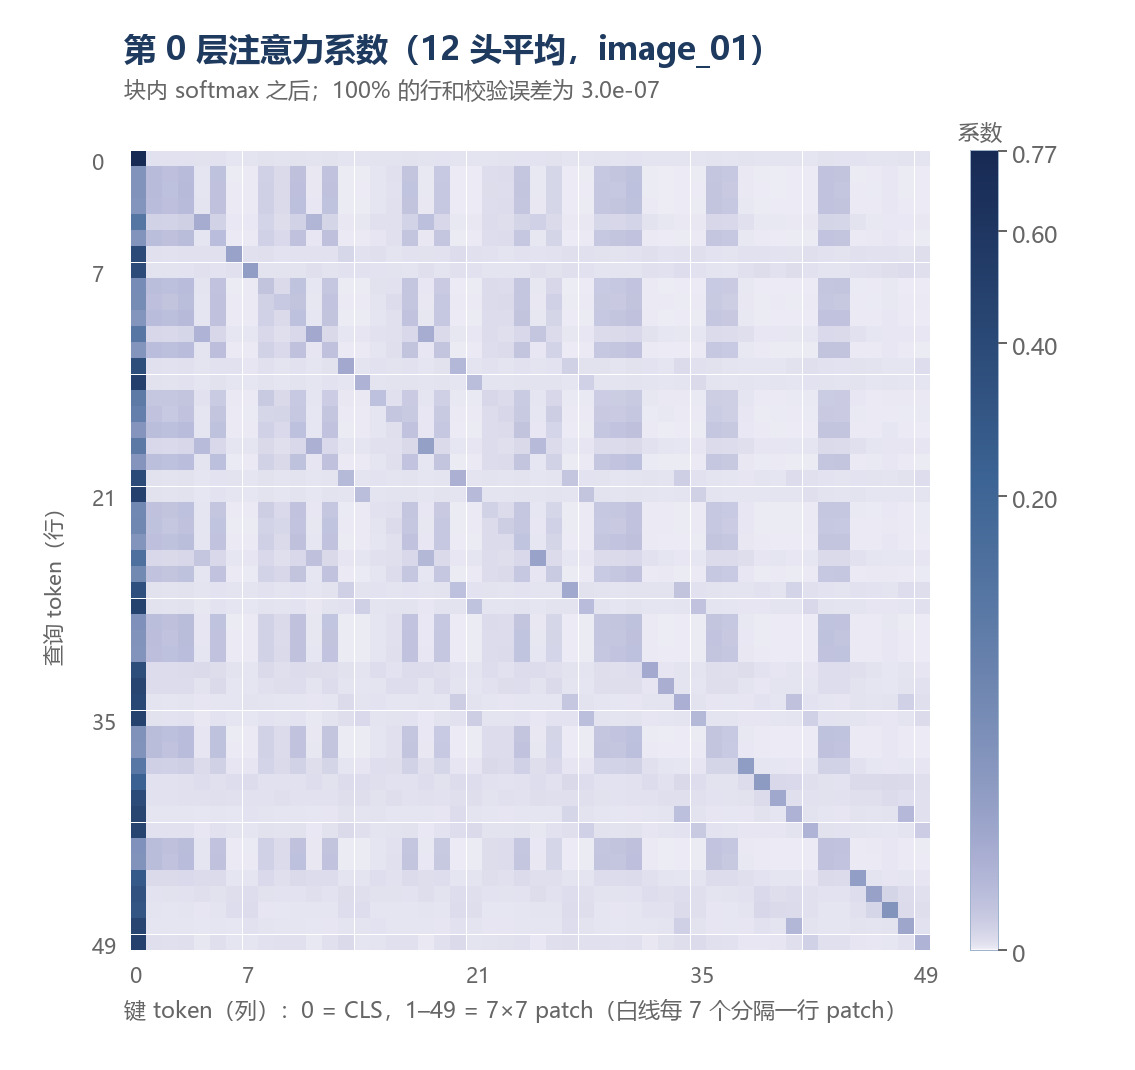
\includegraphics[width=0.58\linewidth]{attention.jpg}
    \caption{第 0 层注意力系数（12 头平均，image\_01）；行和为 1，校验误差 $3.0\times10^{-7}$。}
    \label{fig:attn}
\end{figure}

为验证“每个环节都不可省”，在副本上逐一破坏单个实现决定、其余保持不变，记录该阶段的最大绝对误差
（表~\ref{tab:ablation}）。所有破坏方式的误差都在 $10^{-1}$ 以上，与正确实现的 $10^{-7}$ 量级相差
六个数量级，说明这组结果确实支持“每个环节都必要”的结论，而不只是“程序能跑”。

\begin{table}[H]
\centering
\caption{单点破坏的误差量级（2 张图，output 阶段；patchify 两项为 patches 阶段）}
\label{tab:ablation}
\small
\begin{tabular}{llc}
\hline
破坏方式 & 出现阶段 & max\_abs \\
\hline
patchify 直接 reshape，不转置 & patches & 3.81e+00 \\
patch 内按 H,W,C 展平 & patches & 3.94e+00 \\
残差基准用 $\mathrm{LN}_1(x)$ 而非 $x$ & output & 3.23e-01 \\
ReLU 代替精确 GELU & output & 2.72e-01 \\
CLS 误取 token 1 & output & 2.18e-01 \\
合并头缺少 \texttt{transpose(0,2,1,3)} & output & 1.99e-01 \\
去掉 $1/\sqrt{d_h}$ 缩放 & output & 1.30e-01 \\
正确实现（对照） & output & 4.40e-07 \\
\hline
\end{tabular}
\end{table}

\section{Discussion}

\subsection{一个关键的 shape 变化：patchify 的六维重组}

patchify 把 \texttt{[B,3,224,224]} 变成 \texttt{[B,49,3072]}，必须经过
reshape $\to$ transpose $\to$ reshape 三步。第一步 reshape 为 \texttt{[B,3,7,32,7,32]}，只是给
“网格轴”和“块内轴”命名，不移动任何数值；第二步 transpose 为 \texttt{[B,7,7,3,32,32]}，把网格轴
提到前面、使块内三轴在内存上连续；第三步才能合并为 \texttt{[B,49,3072]}。若省略第二步而直接展平，
每 3072 个数会横跨多行像素与多个通道，得到错误的“块”，实测误差 3.81。块内顺序取 $C,H,W$ 而非
$H,W,C$，是因为 \texttt{conv1} 权重以 \texttt{[768,3,32,32]} 存储并按 $C,H,W$ 展平，两者必须一致，
否则误差 3.94。

\subsection{一个 bug：合并多头时遗漏转置}

现象：形状全程合法、dtype 正确，程序不报错，但 output 阶段 max\_abs 达到 $1.99\times10^{-1}$。
定位依靠分阶段对拍：tokens 阶段通过（$4.39\times10^{-5}$），说明 patchify、投影、CLS 与位置编码都
正确，错误必在 12 个块内部；block0 阶段即失败，说明与层数无关、是单块内部错；再在块内把注意力输出
与逐步手算值对照，锁定在头合并处。根因是 \texttt{split\_heads} 把 $[B,N,H,d_h]$ 转成
$[B,H,N,d_h]$，合并时若直接 reshape 成 $[B,N,H\,d_h]$ 而不先 transpose 回 $[B,N,H,d_h]$，就会把
“不同 token 的同一个头”拼接在一起。修复即补上逆变换并抽出 \texttt{merge\_heads} 方法，误差回到
$4.40\times10^{-7}$。教训是 reshape 与 transpose 必须成对出现，“形状对”不等于“数值对”。

\subsection{局限与改进}

局限：其一，float32 累积偏差从 $10^{-7}$ 增长到 $4\times10^{-5}$，无法与 PyTorch 结果逐位相同；
其二，精确 GELU 由给定 helpers 以 Python 循环逐元素调用 \texttt{math.erf} 实现，是 3.19 s 耗时的
主要来源（10 图 $\times$ 12 块 $\times$ 50 token $\times$ 3072 维）；其三，仅实现视觉塔，未覆盖文本
塔与图文相似度。改进方向：用向量化 erf（或 tanh 近似，注意会改变末位数值）替换逐元素循环；把
12 层的 QKV 线性层拼成一次批量 matmul 以减少 Python 层循环；位置编码与 CLS 广播可预缓存。若重做，
会先为 \texttt{split\_heads}/\texttt{merge\_heads} 写以 arange 构造的单元测试，再拼装整模型，
避免这类“形状对、数值错”的隐性 bug 拖慢调试。

\subsection{贡献与 AI 使用说明}

本人贡献：独立完成六组 TODO 的编码与调试，完成 README、仓库整理与本文数据采集
（\texttt{docs/metrics.json}）；文中所有数值均由本人运行 \texttt{check.py} 与自写度量脚本得到。
参考为课程 PPT 第 46--70 页、附件 \texttt{transformer\_steps.py} 的逐变量演算、NumPy 文档及
OpenCLIP 与 ViT 原论文。

AI 工具使用：本实现与报告初稿在 AI 助手（DeepSeek Harness）辅助下完成，主要用于核对
reshape/transpose 的轴序、解释多头拆分的内存布局与整理文字；其给出的每条建议均通过
\texttt{check.py} 的分阶段对拍验证后才保留，作者可逐行解释实现与数据。

\newpage

% ============================================================
% 批阅与成绩评定页
% ============================================================

\begin{tikzpicture}[remember picture, overlay]
  \draw[thick]
    ($(current page.north west)+(2cm,-3cm)$)
    rectangle
    ($(current page.south east)+(-2cm,3.5cm)$);
\end{tikzpicture}

\vspace{1cm}

\noindent \textbf{指导教师批阅意见：}
\vspace{6cm}
\hfill

\vspace{1cm}

\noindent \textbf{成绩评定：}
\vspace{2cm}
\hfill

\vspace{1cm}

\noindent
\hfill
\textbf{指导教师签字：}\quad\quad\quad\quad\quad\\[0.5cm]

\hfill
\textbf{年}\quad\quad
\textbf{月}\quad\quad
\textbf{日}\quad

\vspace{1cm}

\noindent \textbf{备注：}

\begin{tikzpicture}[remember picture, overlay]
  \node[
    anchor=north west,
    inner sep=0pt,
    text width=\dimexpr\paperwidth-4cm\relax
  ] at ($(current page.south west)+(2cm,3.1cm)$) {
    \begin{minipage}{\dimexpr\paperwidth-4cm\relax}
      \small
      \noindent
      \textbf{注：}\;1、报告内的项目或内容设置，可根据实际情况加以调整和补充。\\[0.2cm]
      \phantom{\textbf{注：}\;}2、教师批改学生实验报告时间应在学生提交实验报告时间后 10 日内。
    \end{minipage}
  };
\end{tikzpicture}

\end{document}
